\begin{figure*}[!t]
\centering
\subfigure[Intent Detection] {
    \label{fig_overview_intent}
    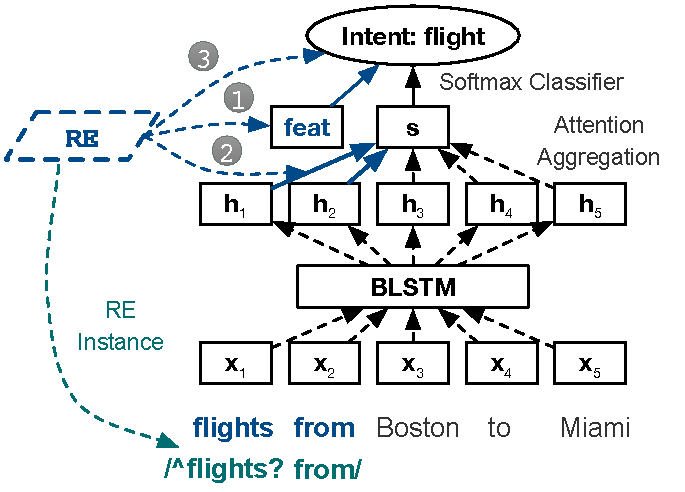
\includegraphics[width=0.8\columnwidth]{figure/re_nn_overview_intent.pdf}
}
\hspace{.5in}
\subfigure[Slot Filling (predicting slot label for \textsl{\underline{Boston}})] {
    \label{fig_overview_slot}
    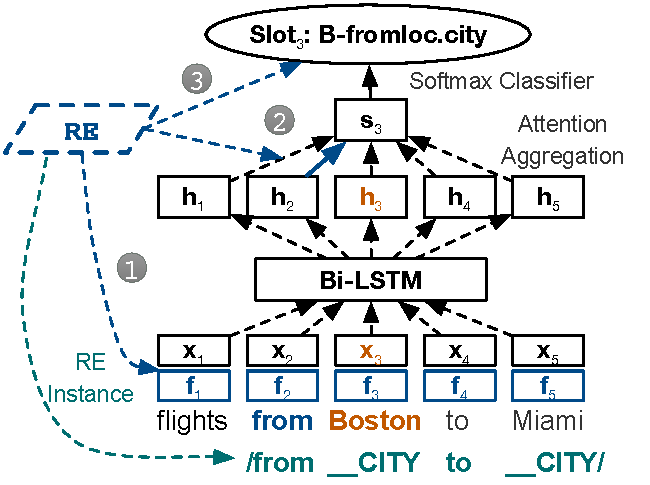
\includegraphics[width=0.8\columnwidth]{figure/re_nn_overview_slot.pdf}
}
\caption{Overview of our methods. \circled{1}, \circled{2}, \circled{3} refers to the methods in
Sec.~\ref{fusion_with_input}, \ref{interact_with_module}, \ref{fusion_with_output} respectively.}
 % and the \RE that applies to the input
% sentence is shown in the bottom.}
\label{fig_overview}
\end{figure*}
\section{Our Approach}
As depicted in Fig.~\ref{fig_overview}, we propose three methods to combine \NN and \REs.
 % for intent detection and slot filling.
% We present each method in the following sub-sections, starting by describing the base \NN model used by all the three methods.

\subsection{Base Models}
We use the Bi-directional LSTM (\BLSTM) as our base \NN model, which is effective in both intent detection and slot
filling~\cite{liu2016attention}.
% Further, to obtain sentence embedding for intent detection, we use a self-attention layer upon the \BLSTM output.

\cparagraph{Intent Detection}
As shown in Fig.~\ref{fig_overview}, given the word embeddings $[\textbf{x}_1, ..., \textbf{x}_n]$ as input, where $n$ is the sentence length, \BLSTM outputs a vector $\textbf{h}_i$ for each word $i$.
Then, we use a self-attention layer to compute the sentence embedding $\textbf{s}$:
\begin{equation}
\textbf{s} = \sum_{i}{\alpha_i\textbf{h}_i}, \quad \alpha_i=\frac{exp(\textbf{h}_i^T\textbf{Wc})}{\sum_{i}{exp(\textbf{h}_i^T\textbf{Wc})}}
\label{eq:simple_att}
\end{equation}
where  $\alpha_i$ is the attention for word $i$, $\textbf{c}$ is a randomly initialized trainable vector used to select informative words for classification, and $\textbf{W}$ is a weight matrix.
Finally, $\textbf{s}$ is fed to a softmax classifier for intent classfication.

\cparagraph{Slot Filling}
The model for slot filling is more straightforward. Given the output of \BLSTM, the slot label prediction of word $i$ is generated by a
softmax classifier which takes $\textbf{h}_i$ as input (the attention aggregation in Fig.~\ref{fig_overview} is used in Sec.~\ref{interact_with_module}).


\subsection{Fusion on the Input Side}
\label{fusion_with_input}
% Similar to the stacking technique \cite{wolpert1992stacked}, a straightforward way to combine \RE and \NN is to use the output of \RE patterns as feature, and feed them as input of \NN models.
On the input side, we use the output of \RE patterns as feature, and feed them as input of \NN models.

\cparagraph{Intent Detection}
Our \REtag for intent detection is the same as the intent label.
% \footnote{If no \RE matches, we will assign a special tag indicating no matches. This process is applied to all the settings.}
Due to the imperfection of the \REs, one sentence may have several \RE tags that may possibly conflict with each other. For example, the
sentence \textsl{\underline{list the delta airlines flights to Miami}} may match a \RE \texttt{/list(\;the)?\;\_\_AIRLINE/} that output
tag \emph{airline}, and another \RE \texttt{/list(\,\textbackslash w+)\{0,3\} flights?/} that output tag \emph{flight}.
% \footnote{\texttt{\_\_WORD} matches a single word, which can be \texttt{/\textbackslash w+/}.}

% Many paper has proved that, embed the discrete feature is an effective method to combine features in \NN \cite{zeng2014relation, guo2017deepfm}.
Since there may exist several \REtags for each sentence, we average the tag embeddings to form an aggregated embedding as input.
Then, there are two ways to add this embedding: (1) append it to the embedding of every input word, (2) append it to the input of the softmax classifier (see \circled{1} in Fig.~\ref{fig_overview_intent}).
% Note that, in the first method, the tag embedding is actually copied $n$ times, where $n$ is the sentence length.
In our pilot experiments on the first method, since the tag embedding is copied many times, the \NN tend to heavily rely on the \REtags, making the fusion performance similar to the performance of \RE alone in few-shot settings. Therefore, we adopt the second method in this paper.

\cparagraph{Slot Filling}
Since the output of slot \RE patterns output word-level tags, as shown in \circled{1} in Fig.~\ref{fig_overview_slot}, we can simply embed
and average the \RE tags into a vector $\textbf{f}_i$ for each word, and append it to the corresponding word embedding $\textbf{w}_i$.
Further, since our slot labels follow the \BIO annotation paradigm, we also extend the slot \RE tags to the \BIO format. For example, the
\REtag of phrase \textsl{\underline{New York}} is \emph{B-city I-city} if its original tag is \emph{city}.

\subsection{Fusion on the NN Module Side}
\label{interact_with_module}
Since the \RE itself has already highlighted the clue words (bold blue arrows and words in \circled{2} of Fig.~\ref{fig_overview}) for its output tag, it can therefore help us guide the attention module in \NN.
% In \circled{2} of Fig.~\ref{fig_overview}, the bold blue arrows and words indicates the clue words marked by \RE.

\cparagraph{Intent Detection}
Taking the sentence in Fig.~\ref{atis_sample} for example, the \RE \texttt{/\textasciicircum flights?\:from/} that leads to intent \emph{flight} means that, \textsl{\underline{flights from}} are key words to decide the intent \emph{flight}. Therefore, the attention module in \NN should attend to these two words to make correct prediction.

Different from the base intent model, we make two changes to better incorporate the guidance from \RE.
First, since each intent has its own clue words, using a single sentence embedding, which is produced by only one set of attention, would make the attention less focused.
% Considering we also know the intent that each \RE points to,
Therefore, we let each intent $i$ use diffenrent attentions $\textbf{a}_i$, which is then used to generate the sentence embedding $\textbf{s}_i$ for that intent specifically:
\begin{equation}
\textbf{s}_i = \sum_{j}{\alpha_{ij}\textbf{h}_j}, \quad
\alpha_{ij}=\frac{exp(\textbf{h}_j^T\textbf{W}_a\textbf{c}_i)}{\sum_{j}{exp(\textbf{h}_j^T\textbf{W}_a\textbf{c}_i)}}
\label{label_att_eq}
\end{equation}
where $\textbf{c}_i$ is a trainable vector for intent $i$ which is used to compute attention $\textbf{a}_i$, $\textbf{h}_j$ is the \BLSTM output for word $j$, and $\textbf{W}_a$ is a weight matrix.

The probability $p_i$ that the input sentence expresses intent $i$ is computed by:
\begin{equation}
p_i = \frac{logit_i}{\sum_{i}{logit_i}}, \quad\quad logit_i=\textbf{w}_i\textbf{s}_i + b_i
\label{label_prob_eq}
\end{equation}
where $\textbf{w}_i$, $logit_i$, $b_i$ are weight vector, logit, and bias for intent $i$ respectively.

Second, apart from indicating a sentence expressing intent $i$ (\textbf{\emph{positive \REs}}), a \RE can also indicate that a sentence does not express intent $i$ (\textbf{\emph{negative \REs}}). Therefore, to make use of negative \REs, we use another set of attentions (\textbf{\emph{negative attentions}}, in contrary to \textbf{\emph{positive attentions}}) to compute a new set of logits for each intent using Eq.~\ref{label_att_eq} and \ref{label_prob_eq}.
By denoting the logits computed by positive attentions as $logit_{pi}$, and the ones computed by negative attentions as $logit_{ni}$, the final logit for intent $i$ is then:
\begin{equation}
logit_i = logit_{pi} - logit_{ni}
\end{equation}

To use \RE patterns to guide the attention, we add an attention loss to the final loss:
\begin{equation}
loss_{att} = \sum_{i}{m_i\sum_{j}{t_{ij}log(\alpha_{ij})}}
\label{att_loss}
\end{equation}
where $t_{ij} = 0$ when none of the matched \REs that lead to intent $i$ mark word $j$ as clue word, otherwise $t_{ij} = 1/k_{i}$ where $k_i$ is the number of clue words
% mark by \RE 
for intent $i$. $m_i$ is a 0-1 indicator that equals 1 when there is a matched \RE that leads to intent $i$. We use Eq.~\ref{att_loss} to compute positive attention loss $loss_{att\_p}$ for positive \REs and negative attention loss $loss_{att\_n}$ for negative ones. The final loss is:
\begin{equation}
loss = loss_{c} + \beta_p loss_{att\_p} + \beta_n loss_{att\_n}
\end{equation}
where $loss_{c}$ is the original classification loss, $\beta_p$ and $\beta_n$ are weights for the two attention losses.

In practice, while with some noise, a positive \RE for intent $i$ can often be negative \REs for other intents. For example, the \RE \texttt{/\textasciicircum flights?\:from/} that leads to intent \emph{flight} also indicates that the sentence should not be labeled as intents like \emph{meal} and \emph{quantity}.
Therefore, we use the positive \REs for intent $i$ as the negative \REs for other intents in our experiments.

\cparagraph{Slot Filling}
While we can apply the same \textbf{\emph{two-side attention}} (positive and negative attention) method as we do in intent prediction, we
face an efficiency problem in slot filling. Since we need to assign a label to each word, if we still compute attention for each slot label, we
will have to compute $2\times L \times n^2$ attention values for one sentence, where $L$ is the number of tags and $n$ is the sentence
length. Considering the \BIO tagging format further doubles the number of tags, this will result in a lot of computation and memory
storage.

Therefore, we use a simplified version of the two-side attention, where all the tags share the same set of positive and negative attention.
Specifically, to predict the slot label of word $i$, we use Eq.~\ref{eq:simple_att} (with $\textbf{c}$ replaced with the \BLSTM output of word $i$) to generate one sentence embedding $\textbf{s}_{pi}$ from positive attention, and another sentence embedding $\textbf{s}_{ni}$ from negative attenion.
The final prediction $\textbf{p}_i$ for word $i$ is then:
\begin{equation}
\begin{split}
\textbf{p}_i = softmax((\textbf{W}_p [\textbf{s}_{pi}; \textbf{h}_i] + \textbf{b}_p) \\- (\textbf{W}_n [\textbf{s}_{ni}; \textbf{h}_i] + \textbf{b}_n))
\end{split}
\end{equation}
where $\textbf{W}_{p}$, $\textbf{W}_{n}$, $\textbf{b}_{p}$, $\textbf{b}_{n}$ are weight matrices and bias vecotrs for positive and negative attention respectively. Here we append the \BLSTM output $\textbf{h}_i$ to $\textbf{s}_{pi}$ and $\textbf{s}_{ni}$ because the word $i$ itself also plays an important part in identifying its slot label.

\subsection{Fusion on the Output Side}
\label{fusion_with_output}
The final type of combination is to use \RE to modify the output of \NN, and the method is the same for the two tasks (see \circled{3} in Fig.~\ref{fig_overview}).

% Therefore, instead using a teach-student framework, this enables us to directly influence the logits of each label in a trainable way, so that we do not need to assign a weight for each pattern, and significantly reduces the number of hyper-parameters.

As mentioned in Section \ref{re_desc}, the slot \RE patterns used in this section only output a simplified version of the slot label.
Since the \REtag is related to the slot label, we can further annotate which slot labels that each \RE will lead to.
% To make connections between the \RE tag and the slot label, we further annotate all the slot labels that the output tag may lead to.
For example, a \RE that outputs tag \emph{city} will lead to three slot labels: \emph{fromloc.city}, \emph{toloc.city}, \emph{stoploc.city}.
% Actually, annotating this kind of connections is not difficult, since the \RE tags are generally somewhat related to the target label that we are trying to predict, otherwise the \RE tags will not be able to provide useful information for the prediction.

Let $z_i$ be a 0-1 indicator of whether at least one \RE pattern that leads to target label $i$ matches the input sentence, then the final logits of label $i$ for the sentence (or a specific word for slot filling) is:
\begin{equation}
logit_i = logit'_i + w_i z_i
\end{equation}
where $logit'_i$ is the logit produced by the original \NN, and $w_i$ is a trainable weight indicating the overall confidence for \REs that lead to label $i$.
Here we do not assign a trainable weight for each \RE because there is a good chance that there are only limited sentences matching a specific \RE.

We modify logit instead of the final probability because logit is an unconstrained real value, which matches $w_i z_i$ better than probability.
Further, when doing model ensembling,
% kagglers have also proved emperically that,
ensembling with logits is emperically often better than with the final probability (see the ensemble version of Juan et al.~\shortcite{juan2016field}), which is also the reason that we operate on logit instead of probability in Sec.~\ref{interact_with_module}.
% Further, if we have strong prior confidence on the patterns, we can also easily incorporate these human-assigned pattern weights by simply multiplying it to $w_i$.
